\documentclass[10pt]{article}
\usepackage[margin=1in]{geometry}
\usepackage{amsmath}
\usepackage{newtxtext,newtxmath}
\usepackage{graphicx}
\usepackage{caption}
\graphicspath{{../figures/}}
\captionsetup{font=small,labelfont=normalfont,labelsep=period}
\renewcommand{\thefigure}{S\arabic{figure}}
\title{Supplementary Material\\[4pt]\large Three Equivalent Routes to Estimating Power Spectra: Averaging, Multitaper, and Smoothing}
\author{Elijah Keldsen, Wolfgang Ganglberger, and M. Brandon Westover}
\date{}
\begin{document}
\maketitle
Figure, table and equation numbers without an ``S'' refer to the main text, whose notation (Section~2.1 there) is used throughout: $R$ is the design resolution, $\alpha=N\Delta R/2$ the time--bandwidth product, $L$ the number of tapers, and widths are in units of $1/(N\Delta)$.

\begin{figure}[!htb]
\centering
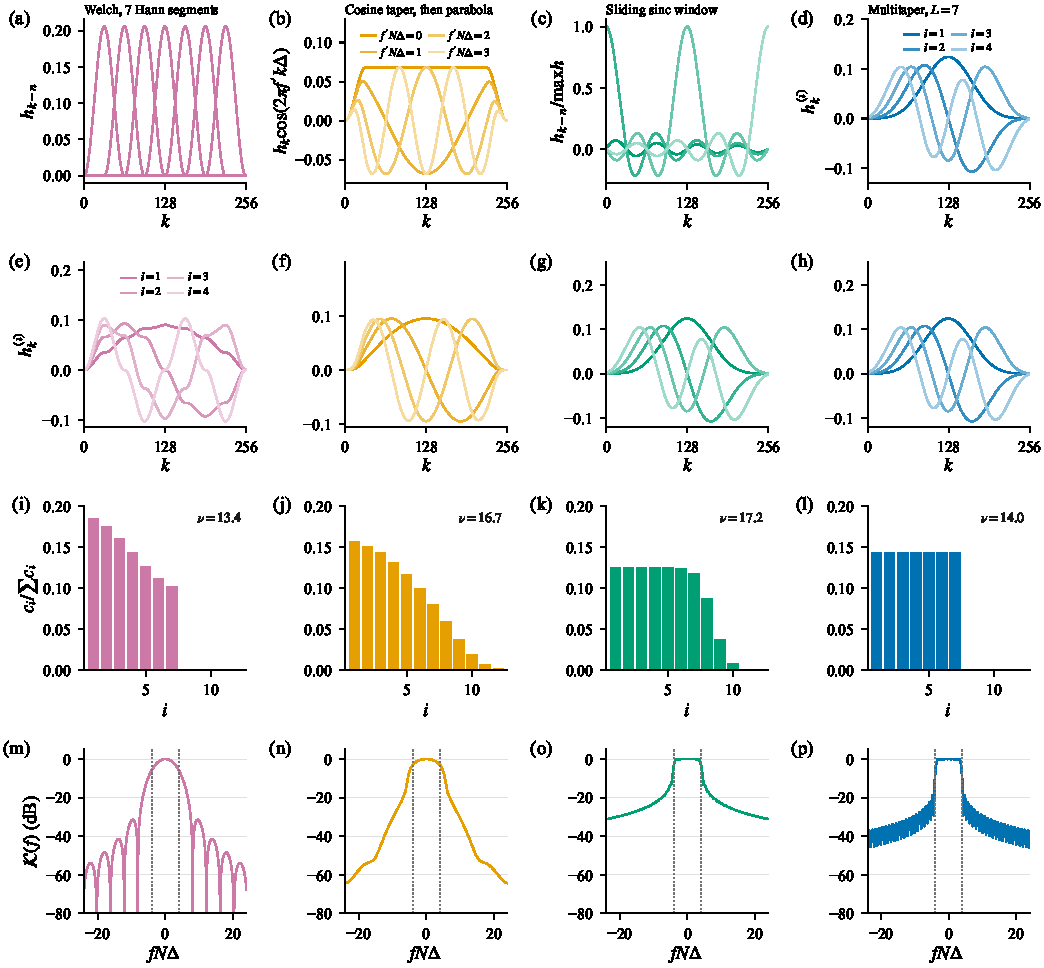
\includegraphics[width=\textwidth]{fig6_taper_banks_full.pdf}
\caption{Fig.~5 in full. Columns and colours as in Fig.~5; rows: the bank as constructed (a--d), the first four eigen-tapers of $Q$ (e--h; for the sliding sinc they are the Slepian sequences, and for Thomson's estimate, whose weights are equal, the Slepians are one of many orthonormal bases of the span), the eigen-weight ladder (i--l), and the kernel in dB relative to its peak (m--p; dotted lines at $|f|=R/2$). The half-power widths of the kernels are 5.84, 8.03, 8.03 and $7.41/(N\Delta)$, and 0.05\%, 0.13\%, 1.39\% and 0.22\% of their power lies outside $|f|\le R$.}
\label{fig:banksfull}
\end{figure}

\begin{figure}[!htb]
\centering
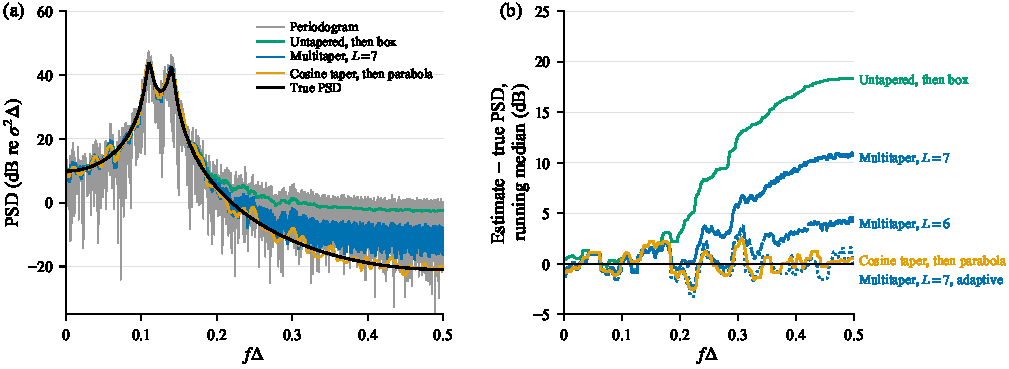
\includegraphics[width=0.8\textwidth]{fig2_ar4_leakage.pdf}
\caption{Dropping the leakiest taper. (a)~One realization of the AR(4) process ($N=1024$, $R=8/(N\Delta)$): the periodogram ($\nu=2$, grey); the untapered periodogram smoothed with the box ($\nu=17.2$, green); the equal-weight multitaper estimate with $L=7$ ($\nu=14$, blue) and with $L=6$ ($\nu=12$, light blue), and the adaptively weighted estimate with $L=7$ (dark blue; its $\nu$ varies with frequency, from 14 where the spectrum is high to 6.5 where it is low); the cosine-tapered periodogram smoothed with a parabola of half-power width $R$ ($\nu=16.7$, orange); and the true PSD (black). Spectra are in dB relative to $\sigma^2\Delta$, where $\sigma^2$ is the variance of the innovations. (b)~Each smoothed estimate minus the true PSD, named at its right-hand end. For $f\Delta\ge0.4$ the untapered box lies 18~dB above the true PSD in the median and the multitaper estimate with $L=7$ lies 10~dB above it. Dropping the seventh taper lowers that to 4~dB, and the adaptive weights and the smoothed periodogram track the truth.}
\label{fig:ar4}
\end{figure}

\begin{figure}[!htb]
\centering
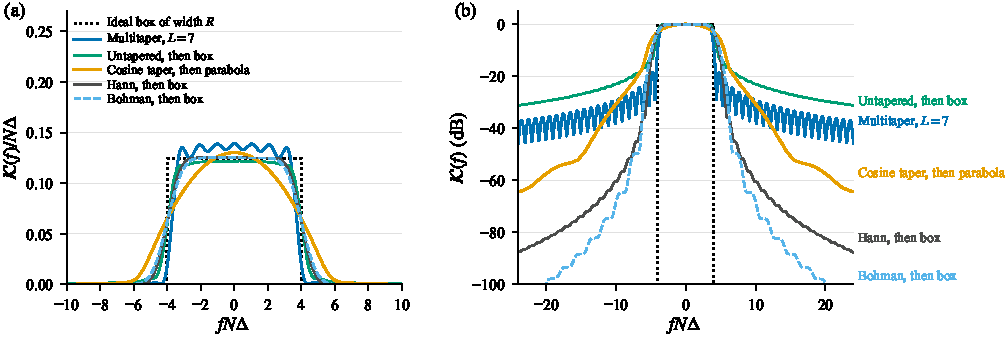
\includegraphics[width=\textwidth]{fig1_kernels.pdf}
\caption{Kernels at the same design resolution ($N=256$, $R=8/(N\Delta)$; Table~2), computed exactly, (a)~on a linear scale near the main lobe and (b)~in dB relative to the peak: the ideal box (dotted); the $L=7$ multitaper kernel ($\nu=14.0$, blue); the periodogram after a 25\% cosine taper followed by a parabola of the same half-power width ($\nu=16.7$, orange), which is recipe (b$'$); and the untapered ($\nu=17.2$, green), Hann ($\nu=8.9$, grey) and Bohman ($\nu=7.3$, light blue, dashed) periodograms followed by the box. In (b) each curve is named at its right-hand end. The half-power widths are $7.4/(N\Delta)$ for the multitaper kernel and $8.0/(N\Delta)$ for the others. At $|f|=12/(N\Delta)$ the skirts lie between $-24$~dB (untapered) and $-75$~dB (Bohman), a range of 51~dB.}
\label{fig:kernels}
\end{figure}

\begin{figure}[!htb]
\centering
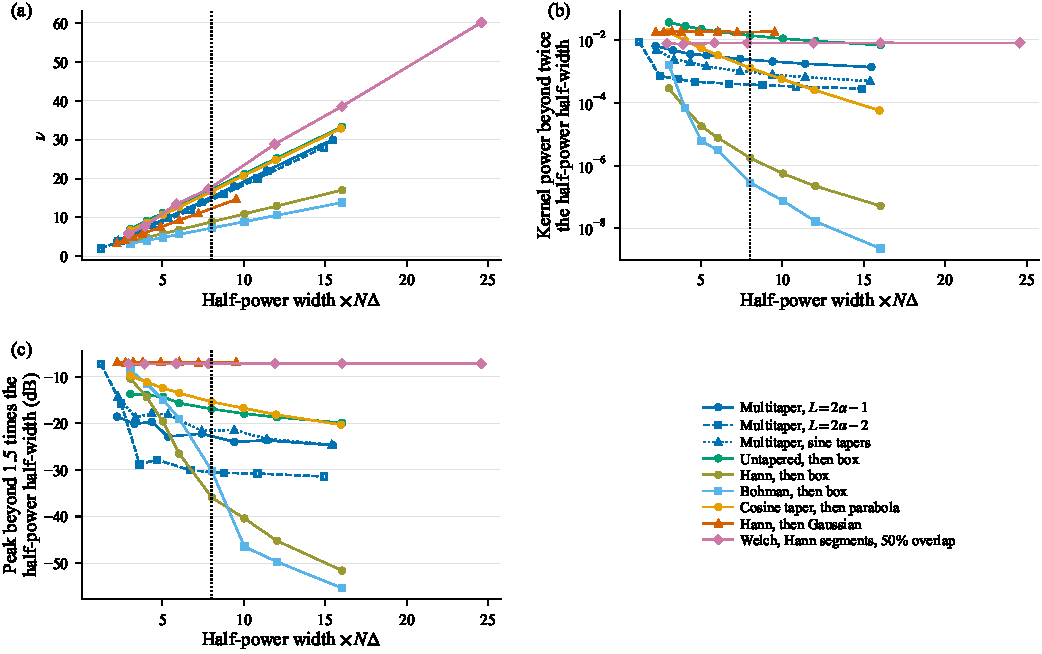
\includegraphics[width=\textwidth]{fig3_tradeoff.pdf}
\caption{Variance, leakage and side-lobe level against the measured resolution, for $N=256$. All curves are exact kernel and degrees-of-freedom computations, with no sampling variability. Each method's bandwidth parameter is swept and the quantities are plotted against the resulting half-power width, so methods are compared at equal resolution: multitaper with $L=2\alpha-1$ and $2\alpha-2$ Slepian tapers and with sine tapers; untapered, Hann and Bohman periodograms followed by a box; a cosine-tapered periodogram followed by a parabola; a Hann periodogram followed by a Gaussian; Welch's method with 50\% overlap. (a)~Equivalent degrees of freedom $\nu$ (higher means less variance). (b)~Kernel power beyond twice the half-power half-width. (c)~The peak of the kernel beyond $1.5\times$ the half-power half-width, in dB relative to its maximum. The Gaussian, parabolic and Welch kernels have no flat top, so for them this quantity is the skirt of the main lobe and not a side lobe, and their markers are filled. The dotted line marks the $8/(N\Delta)$ width of Table~2, and the legend is at the lower right.}
\label{fig:tradeoff}
\end{figure}


\end{document}
